\section{Сравнение различных типов множественных разверток}
  Одним из недостатков использования метода редукции размерности с помощью развёрток является потеря информации о близости точек в многомерном пространстве при
  решении одномерной задачи. На рис. \ref{fig:paraboloid} представлена развертка двухмерного параболоида вращения. Как видно из графика, единственный глобальный уровень расщепился на три.
  \begin{figure}[ht]
  	\center
    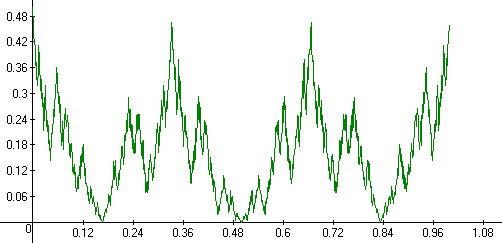
\includegraphics[width=0.55\textwidth]{pictures/map_paraboloid.png}
    \caption{Одномерная функция после подстановки развертки в \(\phi(y)=y_1^2+y_2^2\)}
    \label{fig:paraboloid}
  \end{figure}
   Это происходит из-за того, что развертка может возвращаться в окрестность некоторых точек при разных (далёких друг от друга) значениях одномрного параметра.
   Чтобы частично компенсировать потерю информации о многомерной окрестности точки, были предложены множественные развёртки \cite{shiftedEvolvents, rotatedEvolvents}.
